\section{Background estimation}\label{sec:DataDriven}

\subsection{Estimations with the 2015 data set}

The main background processes that affect this signature arise from non-resonant WW production and from top production, including \ttbar pairs and single top production (mostly tW), and are estimated using data. Instrumental backgrounds arising from misidentified (non-prompt) leptons in W+jets production and mismeasurement of \MET in Drell-Yan events are also estimated from data. The contribution from W$\gamma^*$ is estimated partly from data. The contribution of other sub-dominant backgrounds is obtained directly from simulated samples.

The data-driven background estimation for specific processes is the same as the one described in AN-16-300. In addition, since in this analysis a 2 jets category dedicated to VBF is added, two control regions have been added too to deal with the top and the DY data driven estimations in the 2 jets bin. Moreover the phase space is slightly different with respect to the main \hww analysis.

More precisely top and DY backgrounds normalizations have been extracted direclty from data-simulation comparison in specific control regions enriched in either one or the other backgorund separately for the 0, 1 and 2 jet categories, using the \textit{rateParam} feature of the \textit{combine} package.

Since the DY simulation is different with respect to one used in AN-16-300, new control plots for some variables of interest in the ee and $\mu\mu$ final states are shown in Figs.~\ref{fig:DY_ee} and \ref{fig:DY_mm}.

As also done in the main \hww analysis at 125\GeV, the shape of the \ptll distribution for the DY process is corrected using a reweighting procedure in order to match data. However, differently from the main analysis, here we are using the LO DY sample, thus the reweighting function is slightly different.

Given that this analysis is looking only at different flavor leptons in the final state, this effect is anyway expected to be small in the analysis phase space.

\begin{figure}[htb]
\centering
\subfigure[$\eta$ of leading lepton - ee]{
\includegraphics[width=0.45\textwidth]{Figs/DY/cratio_dyee_13TeV_eta1.png}
}
\subfigure[$\eta$ of trailing lepton - ee]{
\includegraphics[width=0.45\textwidth]{Figs/DY/cratio_dyee_13TeV_eta2.png}
}
\\
\subfigure[\mll - ee]{
\includegraphics[width=0.45\textwidth]{Figs/DY/cratio_dyee_13TeV_mll.png}
}
\subfigure[\ptll - ee]{
\includegraphics[width=0.45\textwidth]{Figs/DY/cratio_dyee_13TeV_ptll.png}
}
\caption{
   Distributions of some variables of interest in a same flavour control region enriched in DY events for the ee final state.}
    \label{fig:DY_ee}
\end{figure}

\begin{figure}[htb]
\centering
\subfigure[$\eta$ of leading lepton - $\mu\mu$]{
\includegraphics[width=0.45\textwidth]{Figs/DY/cratio_dymm_13TeV_eta1.png}
}
\subfigure[$\eta$ of trailing lepton - $\mu\mu$]{
\includegraphics[width=0.45\textwidth]{Figs/DY/cratio_dymm_13TeV_eta2.png}
}
\\
\subfigure[\mll - $\mu\mu$]{
\includegraphics[width=0.45\textwidth]{Figs/DY/cratio_dymm_13TeV_mll.png}
}
\subfigure[\ptll - $\mu\mu$]{
\includegraphics[width=0.45\textwidth]{Figs/DY/cratio_dymm_13TeV_ptll.png}
}
\caption{
   Distributions of some variables of interest in a same flavour control region enriched in DY events for the $\mu\mu$ final state.}
    \label{fig:DY_mm}
\end{figure}

To check the agreement of the DY simulation to the data, a control region has been defined, as close as possible to the signal one, but enriched in Z$\rightarrow$ $\tau^+ \tau^-$ events by selecting a low transverse mass of the two leptons:

\begin{itemize}
\item Leading lepton $\pt > 20$\GeV
\item Trailing lepton $\pt > 20$\GeV
\item No additional leptons with $\pt >10$\GeV (third lepton veto)
\item No jets with p$_T$ $>$ 20~GeV and b-tagging discriminator value $>$ -0.715 (b-veto)
\item $\MET>20$\GeV
\item $\ptll>30$\GeV
\item $\mth<60$\GeV
\item 50~GeV $<$ m$_{\ell\ell}$ $<$ 80~GeV
\end{itemize}

In Fig.~\ref{fig:dy_0jets}, Fig.~\ref{fig:dy_1jet} and Fig.~\ref{fig:dy_2jet} the plots of the Drell Yan enriched control region are shown for events with respectively 0, 1 and 2 jets.\\

\begin{figure}[!h]
\centering
\subfigure[\mt]{
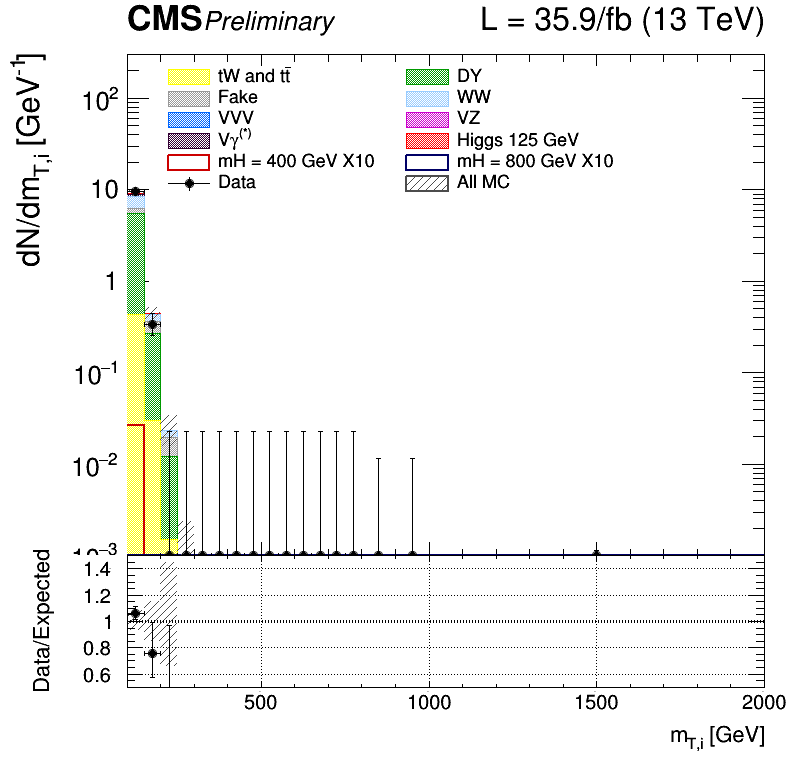
\includegraphics[width=0.44\textwidth]{Figs/DYtt/log_cratio_hww2l2v_13TeV_dytt_of0j_mTi.png}
}
\subfigure[$p_{T,1}$]{
\includegraphics[width=0.44\textwidth]{Figs/DYtt/log_cratio_hww2l2v_13TeV_dytt_of0j_pt1_0j.png}
}\\
\subfigure[$m_{\ell \ell}$]{
\includegraphics[width=0.44\textwidth]{Figs/DYtt/log_cratio_hww2l2v_13TeV_dytt_of0j_mll_0j.png}
}
\subfigure[$p_{T, \ell \ell}$]{
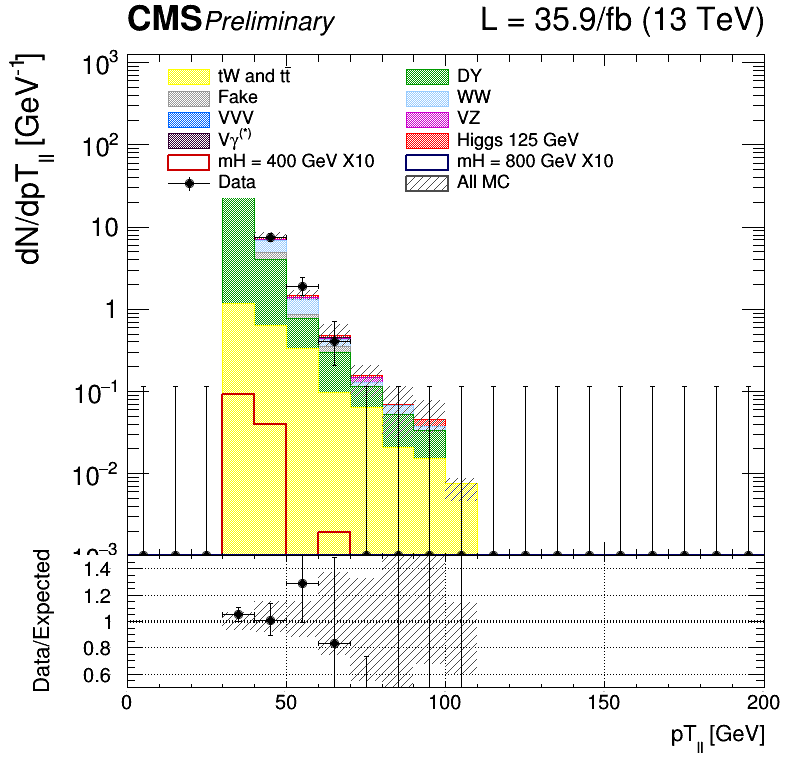
\includegraphics[width=0.44\textwidth]{Figs/DYtt/log_cratio_hww2l2v_13TeV_dytt_of0j_ptll.png}
}
\caption{Control plots for several variables in a Drell-Yan enriched phase space for events with 0 jets with $m_{T}^{H} < 60$~GeV.}\label{fig:dy_0jets}
\end{figure}

\begin{figure}[!h]
\centering
\subfigure[\mt]{
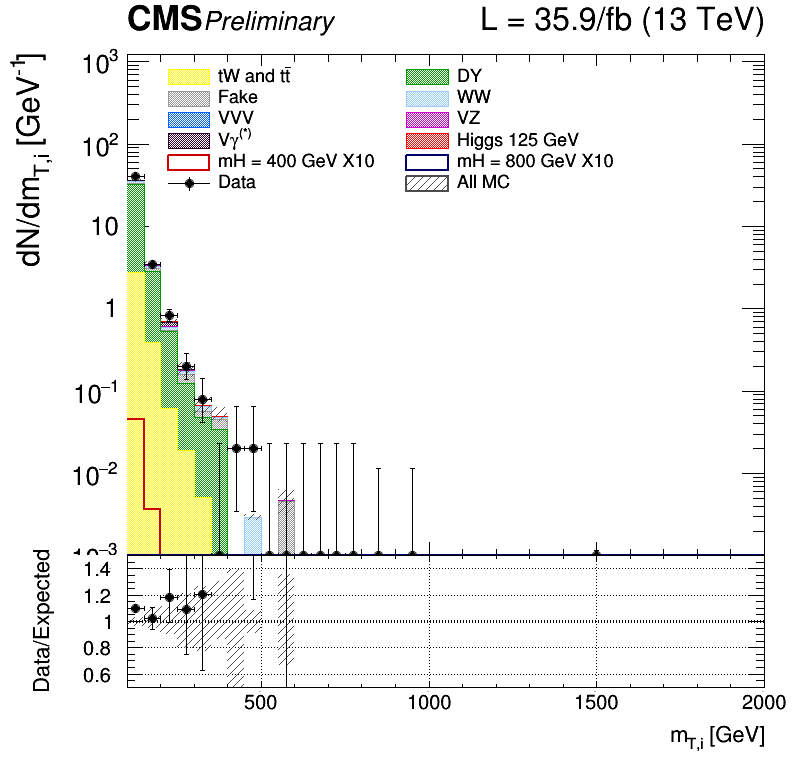
\includegraphics[width=0.44\textwidth]{Figs/DYtt/log_cratio_hww2l2v_13TeV_dytt_of1j_mTi.png}
}
\subfigure[$p_{T,1}$]{
\includegraphics[width=0.44\textwidth]{Figs/DYtt/log_cratio_hww2l2v_13TeV_dytt_of1j_pt1_1j.png}
}\\
\subfigure[$m_{\ell \ell}$]{
\includegraphics[width=0.44\textwidth]{Figs/DYtt/log_cratio_hww2l2v_13TeV_dytt_of1j_mll_1j.png}
}
\subfigure[$p_{T,\ell \ell}$]{
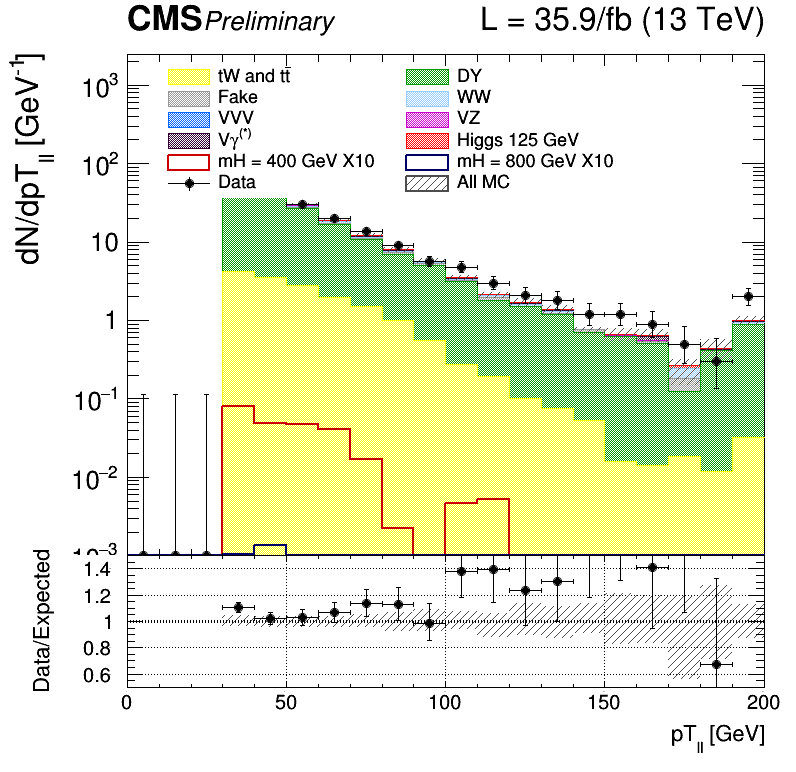
\includegraphics[width=0.44\textwidth]{Figs/DYtt/log_cratio_hww2l2v_13TeV_dytt_of1j_ptll.png}
}
\caption{Control plots for several variables in a Drell-Yan enriched phase space for events with 1 jet with $m_{T}^{H} < 60$~GeV.}\label{fig:dy_1jet}
\end{figure}

\begin{figure}[!h]
\centering
\subfigure[\mt]{
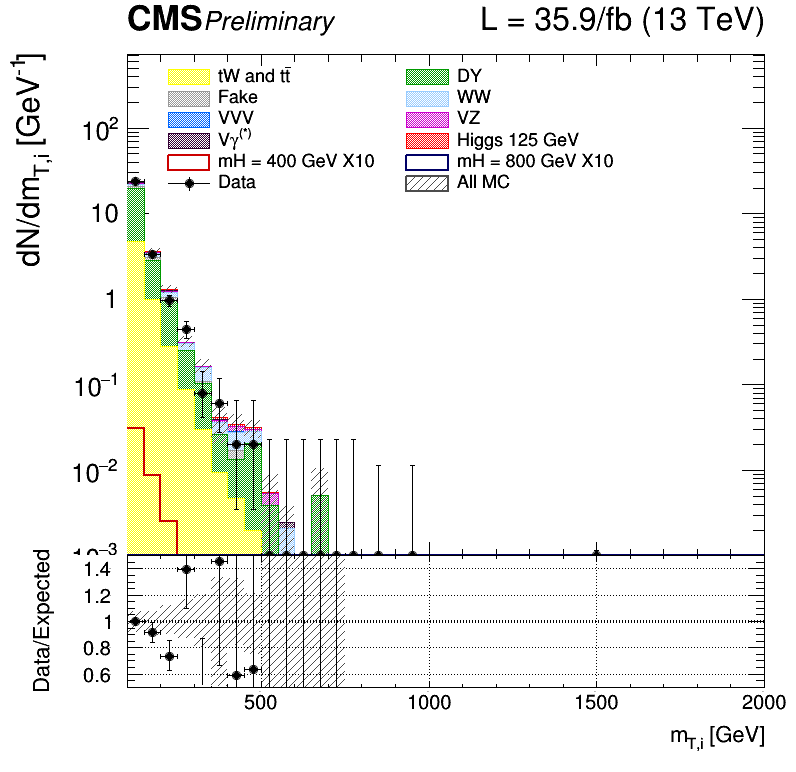
\includegraphics[width=0.44\textwidth]{Figs/DYtt/log_cratio_hww2l2v_13TeV_dytt_of2j_mTi.png}
}
\subfigure[$p_{T,1}$]{
\includegraphics[width=0.44\textwidth]{Figs/DYtt/log_cratio_hww2l2v_13TeV_dytt_of2j_pt1_1j.png}
}\\
\subfigure[$m_{\ell \ell}$]{
\includegraphics[width=0.44\textwidth]{Figs/DYtt/log_cratio_hww2l2v_13TeV_dytt_of2j_mll_2j.png}
}
\subfigure[$p_{T,\ell \ell}$]{
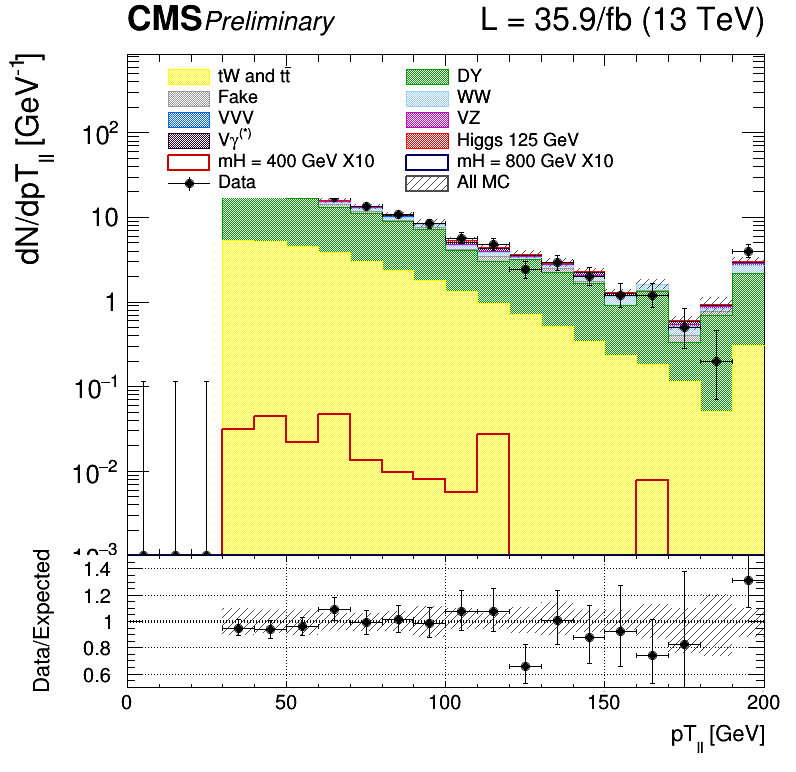
\includegraphics[width=0.44\textwidth]{Figs/DYtt/log_cratio_hww2l2v_13TeV_dytt_of2j_ptll.png}
}
\caption{Control plots for several variables in a Drell-Yan enriched phase space for events with 2 jets with $m_{T}^{H} < 60$~GeV.}\label{fig:dy_2jet}
\end{figure}


To check the agreement of the top background control regions similar to the one in the main \hww analysis have been defined. In particular the control regions are defined requiring the WW level preselections and applying a b-tagging requirement different in the three jet bins:
\begin{itemize}
\item 0 jets bin: at least one b-tagged jet with $20 < \pt < 30$\GeV is required;
\item 1 jet bin: exactly one b-tagged jet with \pt above 30\GeV is required;
\item 2 jets bin: at least one b-tagged jet with \pt above 30\GeV is required.
\end{itemize}

The comparison between data and simulation in the 0 jets control region is shown in Fig.~\ref{fig:top_0jet}. In Fig.~\ref{fig:top_1jet} and Fig.~\ref{fig:top_2jet} are reported the comparisons for the one 1 jet and 2 jets control regions.

\begin{figure}[!h]
\centering
\subfigure[\mt]{
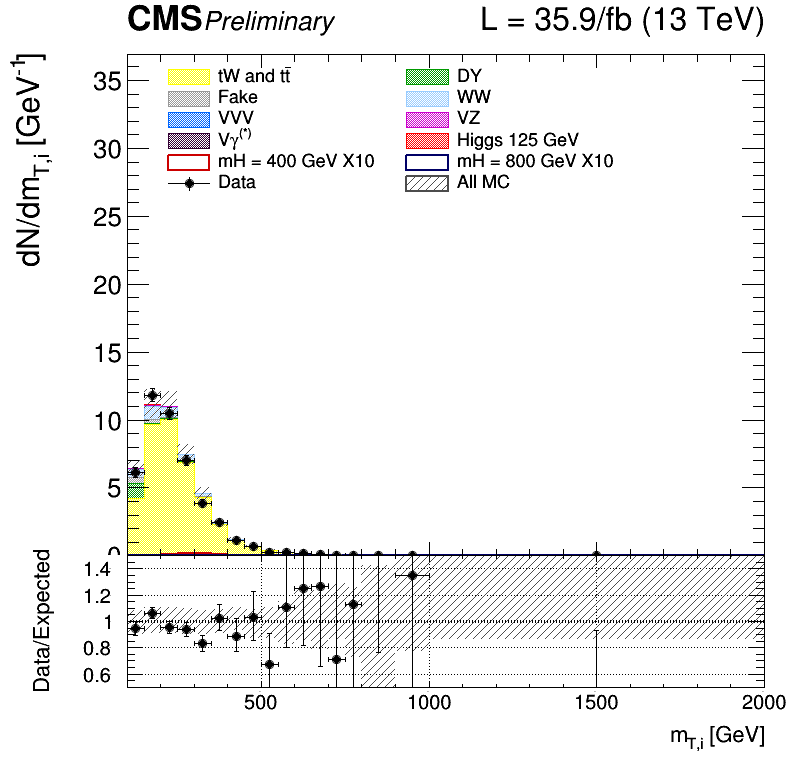
\includegraphics[width=0.45\textwidth]{Figs/Top/2015/cratio_hww2l2v_13TeV_top_of0j_mTi.png}
}
\subfigure[$p_{T,1}$]{
\includegraphics[width=0.45\textwidth]{Figs/Top/2015/cratio_hww2l2v_13TeV_top_of0j_pt1.png}
}\\
\subfigure[$m_{\ell \ell}$]{
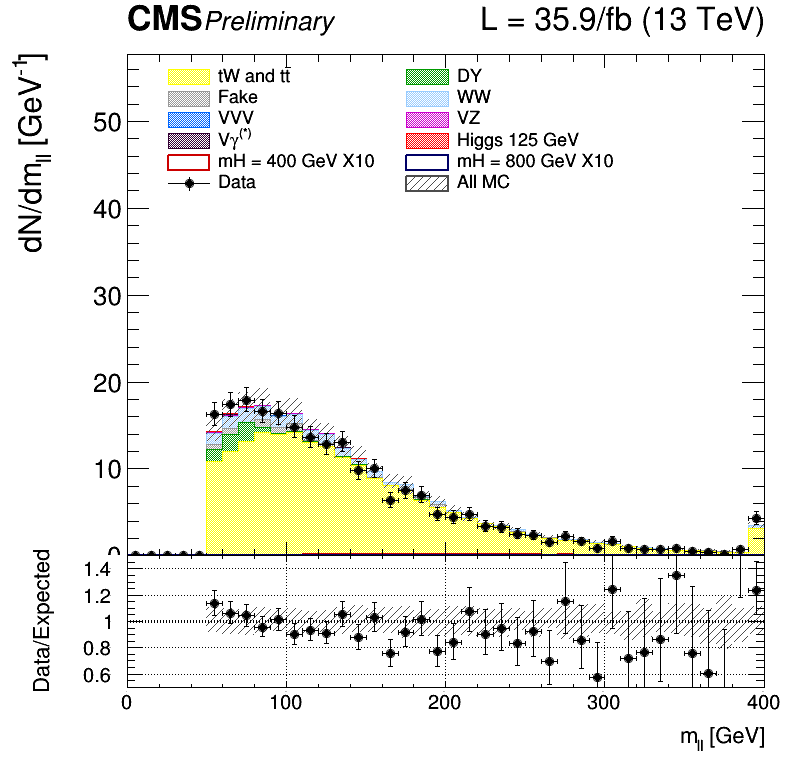
\includegraphics[width=0.45\textwidth]{Figs/Top/2015/cratio_hww2l2v_13TeV_top_of0j_mll.png}
}
\subfigure[$p_{T,\ell \ell}$]{
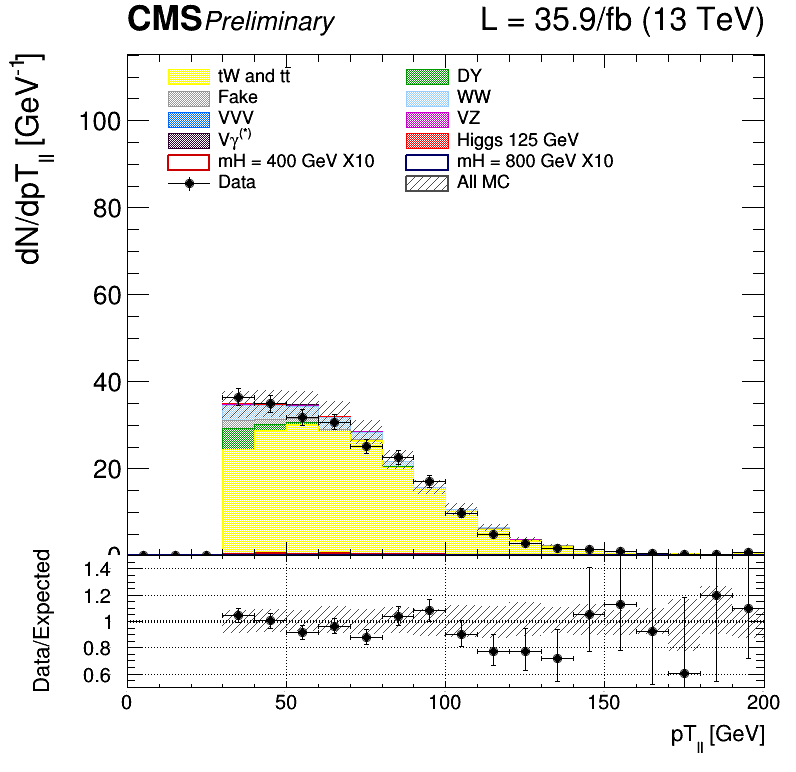
\includegraphics[width=0.45\textwidth]{Figs/Top/2015/cratio_hww2l2v_13TeV_top_of0j_ptll.png}
}
\caption{Control plots for several variables in a top enriched phase space for events with 0 jets and at least one jet with $20 < \pt < 30$\GeV passing the b-tagging requirement.}\label{fig:top_0jet}
\end{figure}

\begin{figure}[!h]
\centering
\subfigure[\mt]{
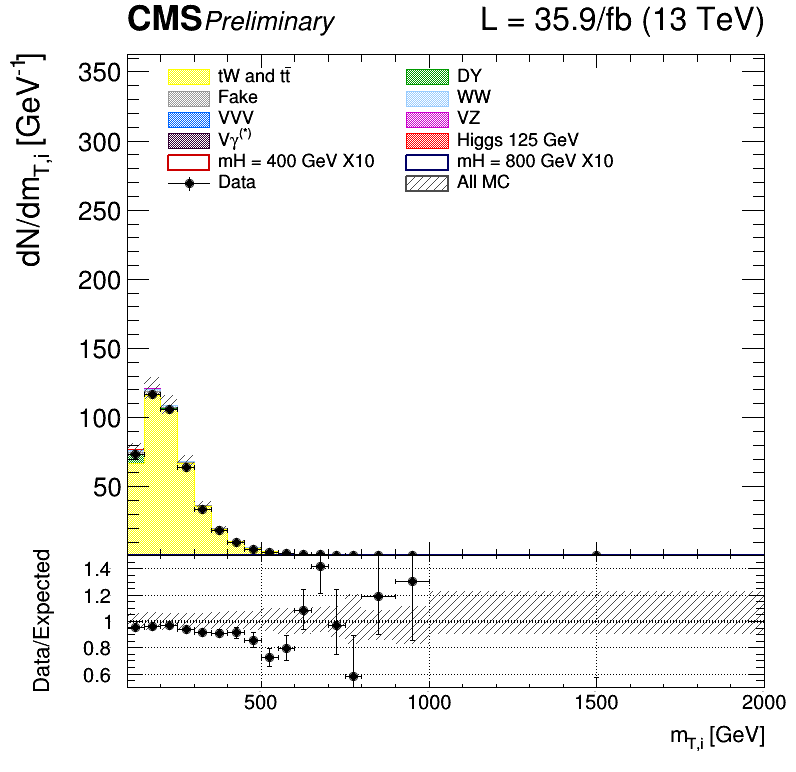
\includegraphics[width=0.45\textwidth]{Figs/Top/2015/cratio_hww2l2v_13TeV_top_of1j_mTi.png}
}
\subfigure[$p_{T,1}$]{
\includegraphics[width=0.45\textwidth]{Figs/Top/2015/cratio_hww2l2v_13TeV_top_of1j_pt1.png}
}\\
\subfigure[$m_{\ell \ell}$]{
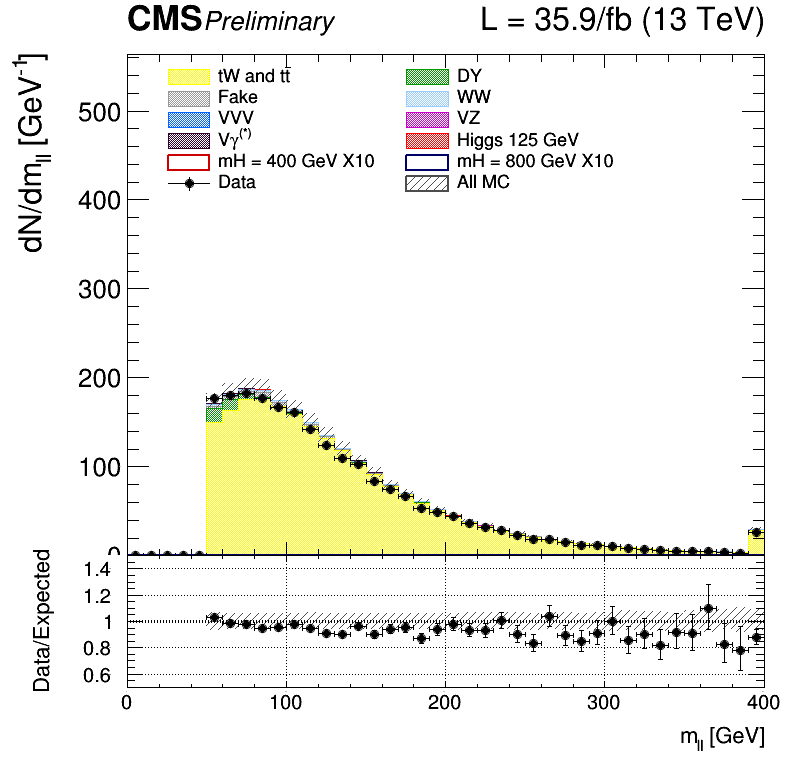
\includegraphics[width=0.45\textwidth]{Figs/Top/2015/cratio_hww2l2v_13TeV_top_of1j_mll.png}
}
\subfigure[$p_{T,\ell \ell}$]{
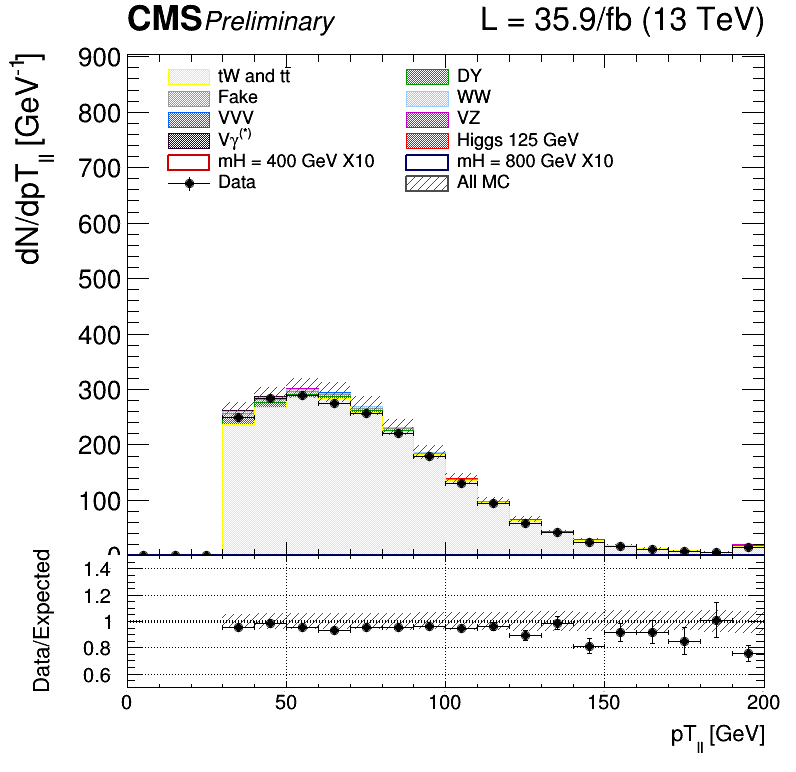
\includegraphics[width=0.45\textwidth]{Figs/Top/2015/cratio_hww2l2v_13TeV_top_of1j_ptll.png}
}
\caption{Control plots for several variables in a top enriched phase space for events with 1 jet and at exactly one jet passing the b-tagging requirement.}\label{fig:top_1jet}
\end{figure}

\begin{figure}[!h]
\centering
\subfigure[\mt]{
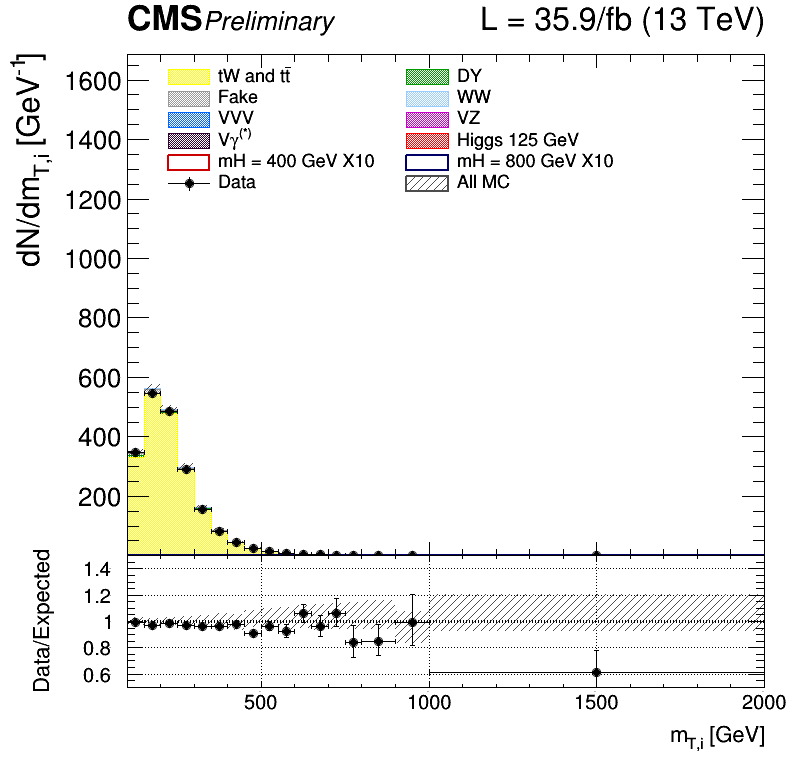
\includegraphics[width=0.45\textwidth]{Figs/Top/2015/cratio_hww2l2v_13TeV_top_of2j_mTi.png}
}
\subfigure[$p_{T,1}$]{
\includegraphics[width=0.45\textwidth]{Figs/Top/2015/cratio_hww2l2v_13TeV_top_of2j_pt1.png}
}\\
\subfigure[$m_{\ell \ell}$]{
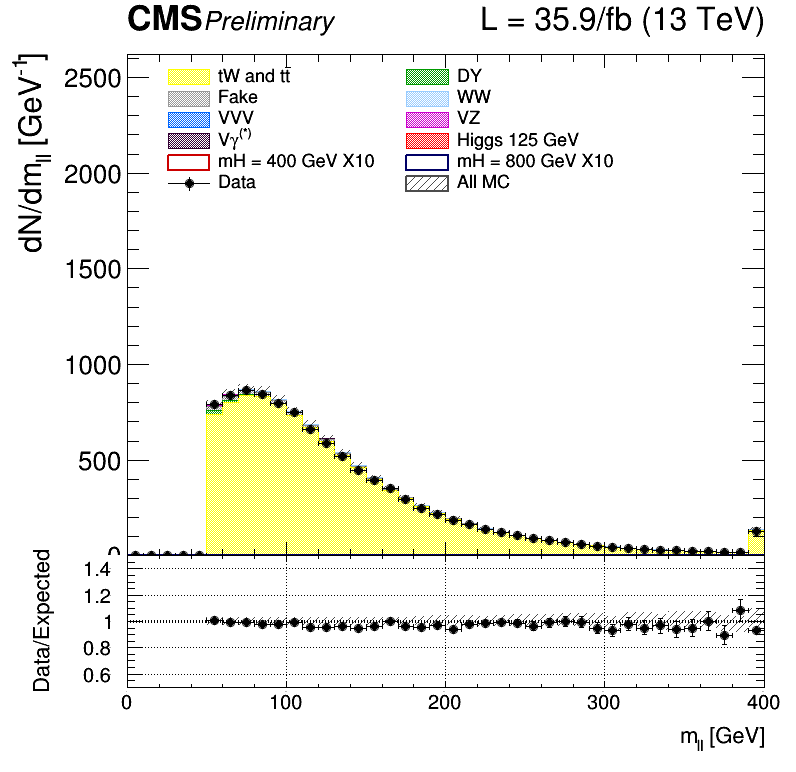
\includegraphics[width=0.45\textwidth]{Figs/Top/2015/cratio_hww2l2v_13TeV_top_of2j_mll.png}
}
\subfigure[$p_{T,\ell \ell}$]{
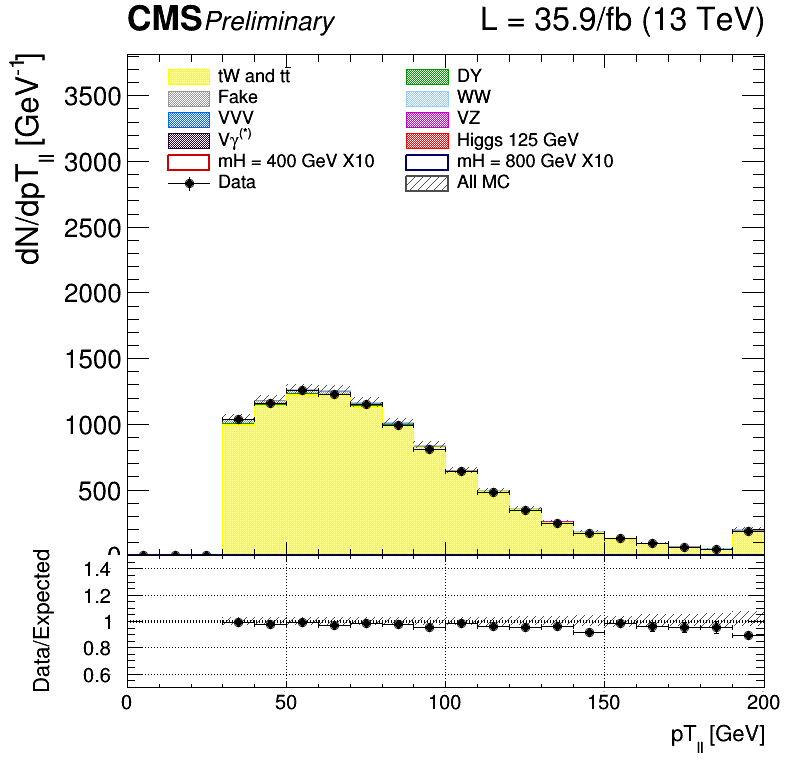
\includegraphics[width=0.45\textwidth]{Figs/Top/2015/cratio_hww2l2v_13TeV_top_of2j_ptll.png}
}
\caption{Control plots for several variables in a top enriched phase space for events with 2 jets and at least one jet passing the b-tagging requirement.}\label{fig:top_2jet}
\end{figure}


To check the agreement with data for the Fake background a same sign dilepton control region has been defined, applying the same requirements as the analysis selections but with two same charge and opposite flavor leptons. The plots for some variables of interest are shown if Figs.~\ref{fig:samesign_0j}, ~\ref{fig:samesign_1j},~\ref{fig:samesign_2j} separately for the three jet categories.

\begin{figure}[!h]
\centering
\subfigure[\mt]{
\includegraphics[width=0.45\textwidth]{Figs/SameSign/2015/cratio_hww2l2v_13TeV_ss_of0j_mTi.png}
}
\subfigure[$p_{T,1}$]{
\includegraphics[width=0.45\textwidth]{Figs/SameSign/2015/cratio_hww2l2v_13TeV_ss_of0j_pt1.png}
}\\
\subfigure[$m_{\ell \ell}$]{
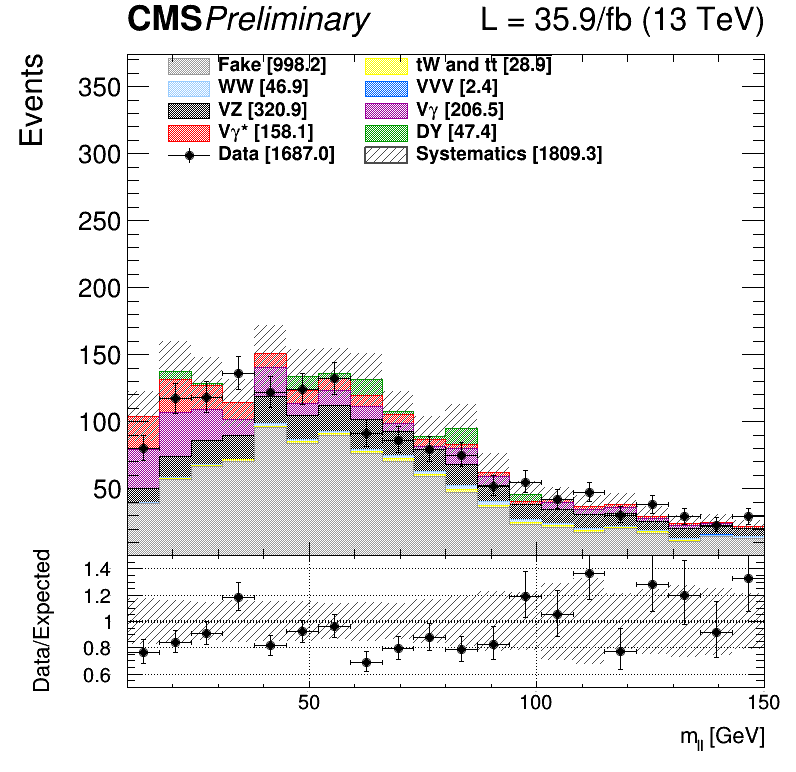
\includegraphics[width=0.45\textwidth]{Figs/SameSign/2015/cratio_hww2l2v_13TeV_ss_of0j_mll.png}
}
\subfigure[$p_{T,\ell \ell}$]{
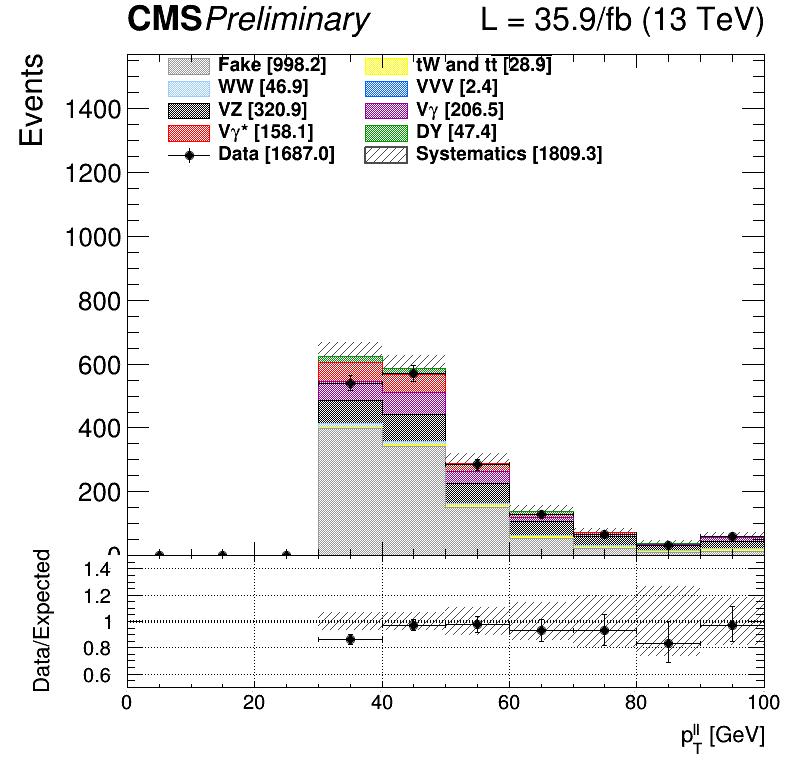
\includegraphics[width=0.45\textwidth]{Figs/SameSign/2015/cratio_hww2l2v_13TeV_ss_of0j_ptll.png}
}
\caption{Control plots for several variables in a same sign dilepton enriched phase space for events with 0 jets.}\label{fig:samesign_0jet}
\end{figure}

\begin{figure}[!h]
\centering
\subfigure[\mt]{
\includegraphics[width=0.45\textwidth]{Figs/SameSign/2015/cratio_hww2l2v_13TeV_ss_of1j_mTi.png}
}
\subfigure[$p_{T,1}$]{
\includegraphics[width=0.45\textwidth]{Figs/SameSign/2015/cratio_hww2l2v_13TeV_ss_of1j_pt1.png}
}\\
\subfigure[$m_{\ell \ell}$]{
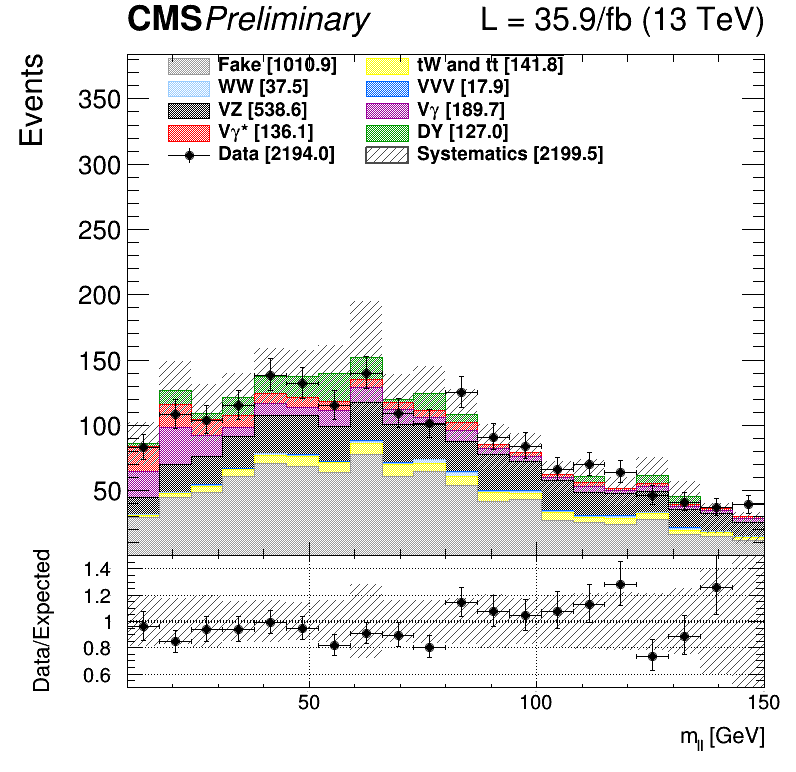
\includegraphics[width=0.45\textwidth]{Figs/SameSign/2015/cratio_hww2l2v_13TeV_ss_of1j_mll.png}
}
\subfigure[$p_{T,\ell \ell}$]{
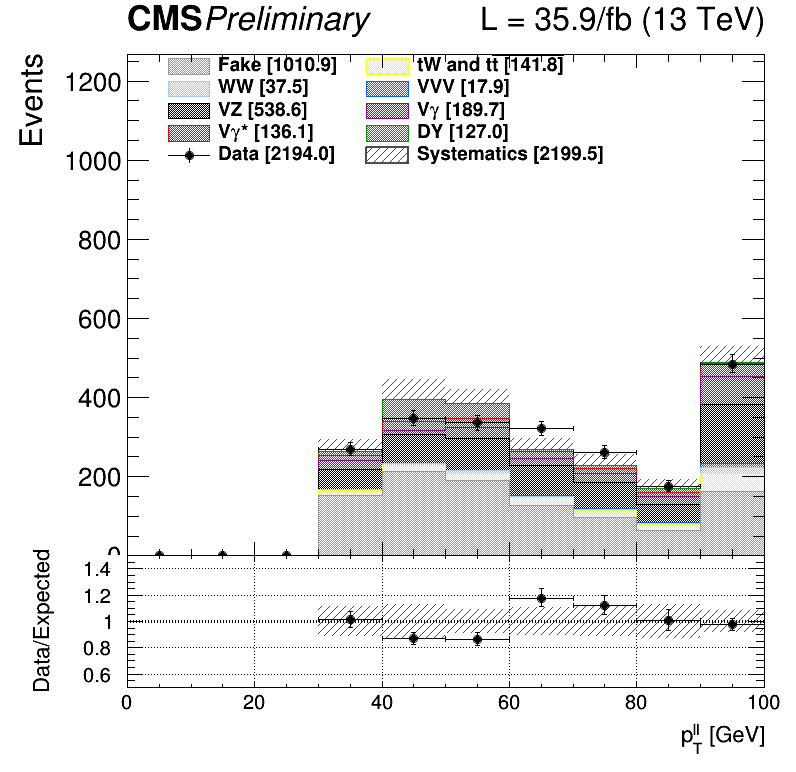
\includegraphics[width=0.45\textwidth]{Figs/SameSign/2015/cratio_hww2l2v_13TeV_ss_of1j_ptll.png}
}
\caption{Control plots for several variables in a same sign dilepton enriched phase space for events with 1 jet.}\label{fig:samesign_1jet}
\end{figure}

\begin{figure}[!h]
\centering
\subfigure[\mt]{
\includegraphics[width=0.45\textwidth]{Figs/SameSign/2015/cratio_hww2l2v_13TeV_ss_of2j_mTi_VBF.png}
}
\subfigure[$p_{T,1}$]{
\includegraphics[width=0.45\textwidth]{Figs/SameSign/2015/cratio_hww2l2v_13TeV_ss_of2j_pt1.png}
}\\
\subfigure[$m_{\ell \ell}$]{
\includegraphics[width=0.45\textwidth]{Figs/SameSign/2015/cratio_hww2l2v_13TeV_ss_of2j_mll.png}
}
\subfigure[$p_{T,\ell \ell}$]{
\includegraphics[width=0.45\textwidth]{Figs/SameSign/2015/cratio_hww2l2v_13TeV_ss_of2j_ptll.png}
}
\caption{Control plots for several variables in a same sign dilepton enriched phase space for events with 2 jets.}\label{fig:samesign_2jet}
\end{figure}




















\clearpage




\subsection{Estimations with the 2016 data set}

The same control regions defined before have been also used to test the agreement of simulation and 2016 data, corresponding to an integrated luminosity of 6.3\ifb.

In Figs.~\ref{fig:DY_ee_2016} and \ref{fig:DY_mm_2016} the distributions of some variables of interest in the same flavor Drell Yan enriched region are shown, separately for the ee and $\mu\mu$ final states.

In Fig.~\ref{fig:dy_0jets_2016}, Fig.~\ref{fig:dy_1jet_2016} and Fig.~\ref{fig:dy_2jet_2016} the plots of the Drell Yan to $\tau\tau$ enriched control region are shown for events with respectively 0, 1 and 2 jets.\\


\begin{figure}[htb]
\centering
\subfigure[$\eta$ of leading lepton - ee]{
\includegraphics[width=0.45\textwidth]{Figs/DY/2016/cratio_dyee_13TeV_eta1.png}
}
\subfigure[$\eta$ of trailing lepton - ee]{
\includegraphics[width=0.45\textwidth]{Figs/DY/2016/cratio_dyee_13TeV_eta2.png}
}
\\
\subfigure[\mll - ee]{
\includegraphics[width=0.45\textwidth]{Figs/DY/2016/cratio_dyee_13TeV_mll.png}
}
\subfigure[\ptll - ee]{
\includegraphics[width=0.45\textwidth]{Figs/DY/2016/cratio_dyee_13TeV_ptll.png}
}
\caption{
   Distributions of some variables of interest in a same flavour control region enriched in DY events for the ee final state.}
    \label{fig:DY_ee}
\end{figure}

\begin{figure}[htb]
\centering
\subfigure[$\eta$ of leading lepton - $\mu\mu$]{
\includegraphics[width=0.45\textwidth]{Figs/DY/2016/cratio_dymm_13TeV_eta1.png}
}
\subfigure[$\eta$ of trailing lepton - $\mu\mu$]{
\includegraphics[width=0.45\textwidth]{Figs/DY/2016/cratio_dymm_13TeV_eta2.png}
}
\\
\subfigure[\mll - $\mu\mu$]{
\includegraphics[width=0.45\textwidth]{Figs/DY/2016/cratio_dymm_13TeV_mll.png}
}
\subfigure[\ptll - $\mu\mu$]{
\includegraphics[width=0.45\textwidth]{Figs/DY/2016/cratio_dymm_13TeV_ptll.png}
}
\caption{
   Distributions of some variables of interest in a same flavour control region enriched in DY events for the $\mu\mu$ final state.}
    \label{fig:DY_mm}
\end{figure}






\begin{figure}[!h]
\centering
\subfigure[\mt]{
\includegraphics[width=0.44\textwidth]{Figs/DYtt/2016/log_cratio_hww2l2v_13TeV_dytt_of0j_mTi.png}
}
\subfigure[$p_{T,1}$]{
\includegraphics[width=0.44\textwidth]{Figs/DYtt/2016/log_cratio_hww2l2v_13TeV_dytt_of0j_pt1_0j.png}
}\\
\subfigure[$m_{\ell \ell}$]{
\includegraphics[width=0.44\textwidth]{Figs/DYtt/2016/log_cratio_hww2l2v_13TeV_dytt_of0j_mll_0j.png}
}
\subfigure[$p_{T, \ell \ell}$]{
\includegraphics[width=0.44\textwidth]{Figs/DYtt/2016/log_cratio_hww2l2v_13TeV_dytt_of0j_ptll.png}
}
\caption{Control plots for several variables in a Drell-Yan enriched phase space for events with 0 jets with $m_{T}^{H} < 60$~GeV.}\label{fig:dy_0jets_2016}
\end{figure}

\begin{figure}[!h]
\centering
\subfigure[\mt]{
\includegraphics[width=0.44\textwidth]{Figs/DYtt/2016/log_cratio_hww2l2v_13TeV_dytt_of1j_mTi.png}
}
\subfigure[$p_{T,1}$]{
\includegraphics[width=0.44\textwidth]{Figs/DYtt/2016/log_cratio_hww2l2v_13TeV_dytt_of1j_pt1_1j.png}
}\\
\subfigure[$m_{\ell \ell}$]{
\includegraphics[width=0.44\textwidth]{Figs/DYtt/2016/log_cratio_hww2l2v_13TeV_dytt_of1j_mll_1j.png}
}
\subfigure[$p_{T,\ell \ell}$]{
\includegraphics[width=0.44\textwidth]{Figs/DYtt/2016/log_cratio_hww2l2v_13TeV_dytt_of1j_ptll.png}
}
\caption{Control plots for several variables in a Drell-Yan enriched phase space for events with 1 jet with $m_{T}^{H} < 60$~GeV.}\label{fig:dy_1jet_2016}
\end{figure}

\begin{figure}[!h]
\centering
\subfigure[\mt]{
\includegraphics[width=0.44\textwidth]{Figs/DYtt/2016/log_cratio_hww2l2v_13TeV_dytt_of2j_mTi.png}
}
\subfigure[$p_{T,1}$]{
\includegraphics[width=0.44\textwidth]{Figs/DYtt/2016/log_cratio_hww2l2v_13TeV_dytt_of2j_pt1_1j.png}
}\\
\subfigure[$m_{\ell \ell}$]{
\includegraphics[width=0.44\textwidth]{Figs/DYtt/2016/log_cratio_hww2l2v_13TeV_dytt_of2j_mll_2j.png}
}
\subfigure[$p_{T,\ell \ell}$]{
\includegraphics[width=0.44\textwidth]{Figs/DYtt/2016/log_cratio_hww2l2v_13TeV_dytt_of2j_ptll.png}
}
\caption{Control plots for several variables in a Drell-Yan enriched phase space for events with 2 jets with $m_{T}^{H} < 60$~GeV.}\label{fig:dy_2jet_2016}
\end{figure}


For the top background the comparison between data and simulation in the 0 jets control region is shown in Fig.~\ref{fig:top_0jet_2016}. In Fig.~\ref{fig:top_1jet_2016} and Fig.~\ref{fig:top_2jet_2016} are reported the comparisons for the one 1 jet and 2 jets control regions.



\begin{figure}[!h]
\centering
\subfigure[\mt]{
\includegraphics[width=0.45\textwidth]{Figs/Top/2016/cratio_hww2l2v_13TeV_top_of0j_mTi.png}
}
\subfigure[$p_{T,1}$]{
\includegraphics[width=0.45\textwidth]{Figs/Top/2016/cratio_hww2l2v_13TeV_top_of0j_pt1.png}
}\\
\subfigure[$m_{\ell \ell}$]{
\includegraphics[width=0.45\textwidth]{Figs/Top/2016/cratio_hww2l2v_13TeV_top_of0j_mll.png}
}
\subfigure[$p_{T,\ell \ell}$]{
\includegraphics[width=0.45\textwidth]{Figs/Top/2016/cratio_hww2l2v_13TeV_top_of0j_ptll.png}
}
\caption{Control plots for several variables in a top enriched phase space for events with 0 jets and at least one jet with $20 < \pt < 30$\GeV passing the b-tagging requirement.}\label{fig:top_0jet_2016}
\end{figure}

\begin{figure}[!h]
\centering
\subfigure[\mt]{
\includegraphics[width=0.45\textwidth]{Figs/Top/2016/cratio_hww2l2v_13TeV_top_of1j_mTi.png}
}
\subfigure[$p_{T,1}$]{
\includegraphics[width=0.45\textwidth]{Figs/Top/2016/cratio_hww2l2v_13TeV_top_of1j_pt1.png}
}\\
\subfigure[$m_{\ell \ell}$]{
\includegraphics[width=0.45\textwidth]{Figs/Top/2016/cratio_hww2l2v_13TeV_top_of1j_mll.png}
}
\subfigure[$p_{T,\ell \ell}$]{
\includegraphics[width=0.45\textwidth]{Figs/Top/2016/cratio_hww2l2v_13TeV_top_of1j_ptll.png}
}
\caption{Control plots for several variables in a top enriched phase space for events with 1 jet and at exactly one jet passing the b-tagging requirement.}\label{fig:top_1jet_2016}
\end{figure}

\begin{figure}[!h]
\centering
\subfigure[\mt]{
\includegraphics[width=0.45\textwidth]{Figs/Top/2016/cratio_hww2l2v_13TeV_top_of2j_mTi.png}
}
\subfigure[$p_{T,1}$]{
\includegraphics[width=0.45\textwidth]{Figs/Top/2016/cratio_hww2l2v_13TeV_top_of2j_pt1.png}
}\\
\subfigure[$m_{\ell \ell}$]{
\includegraphics[width=0.45\textwidth]{Figs/Top/2016/cratio_hww2l2v_13TeV_top_of2j_mll.png}
}
\subfigure[$p_{T,\ell \ell}$]{
\includegraphics[width=0.45\textwidth]{Figs/Top/2016/cratio_hww2l2v_13TeV_top_of2j_ptll.png}
}
\caption{Control plots for several variables in a top enriched phase space for events with 2 jets and at least one jet passing the b-tagging requirement.}\label{fig:top_2jet_2016}
\end{figure}


To check the agreement with data for the Fake background a same sign dilepton control region has been defined, applying the same requirements as the analysis selections but with two same charge and opposite flavor leptons. The plots for some variables of interest are shown if Figs.~\ref{fig:samesign_0j_2016}, ~\ref{fig:samesign_1j_2016},~\ref{fig:samesign_2j_2016} separately for the three jet categories.

\begin{figure}[!h]
\centering
\subfigure[\mt]{
\includegraphics[width=0.45\textwidth]{Figs/SameSign/2016/cratio_hww2l2v_13TeV_ss_of0j_mTi_0j.png}
}
\subfigure[$p_{T,1}$]{
\includegraphics[width=0.45\textwidth]{Figs/SameSign/2016/cratio_hww2l2v_13TeV_ss_of0j_pt1.png}
}\\
\subfigure[$m_{\ell \ell}$]{
\includegraphics[width=0.45\textwidth]{Figs/SameSign/2016/cratio_hww2l2v_13TeV_ss_of0j_mll.png}
}
\subfigure[$p_{T,\ell \ell}$]{
\includegraphics[width=0.45\textwidth]{Figs/SameSign/2016/cratio_hww2l2v_13TeV_ss_of0j_ptll.png}
}
\caption{Control plots for several variables in a same sign dilepton enriched phase space for events with 0 jets.}\label{fig:samesign_0jet_2016}
\end{figure}

\begin{figure}[!h]
\centering
\subfigure[\mt]{
\includegraphics[width=0.45\textwidth]{Figs/SameSign/2016/cratio_hww2l2v_13TeV_ss_of1j_mTi_1j.png}
}
\subfigure[$p_{T,1}$]{
\includegraphics[width=0.45\textwidth]{Figs/SameSign/2016/cratio_hww2l2v_13TeV_ss_of1j_pt1.png}
}\\
\subfigure[$m_{\ell \ell}$]{
\includegraphics[width=0.45\textwidth]{Figs/SameSign/2016/cratio_hww2l2v_13TeV_ss_of1j_mll.png}
}
\subfigure[$p_{T,\ell \ell}$]{
\includegraphics[width=0.45\textwidth]{Figs/SameSign/2016/cratio_hww2l2v_13TeV_ss_of1j_ptll.png}
}
\caption{Control plots for several variables in a same sign dilepton enriched phase space for events with 1 jet.}\label{fig:samesign_1jet_2016}
\end{figure}

\begin{figure}[!h]
\centering
\subfigure[\mt]{
\includegraphics[width=0.45\textwidth]{Figs/SameSign/2016/cratio_hww2l2v_13TeV_ss_of2j_mTi_VBF.png}
}
\subfigure[$p_{T,1}$]{
\includegraphics[width=0.45\textwidth]{Figs/SameSign/2016/cratio_hww2l2v_13TeV_ss_of2j_pt1.png}
}\\
\subfigure[$m_{\ell \ell}$]{
\includegraphics[width=0.45\textwidth]{Figs/SameSign/2016/cratio_hww2l2v_13TeV_ss_of2j_mll.png}
}
\subfigure[$p_{T,\ell \ell}$]{
\includegraphics[width=0.45\textwidth]{Figs/SameSign/2016/cratio_hww2l2v_13TeV_ss_of2j_ptll.png}
}
\caption{Control plots for several variables in a same sign dilepton enriched phase space for events with 2 jets.}\label{fig:samesign_2jet_2016}
\end{figure}








